\documentclass[12pt,a4paper]{article}

% --- Pakiety ---
\usepackage[a4paper, margin=2cm]{geometry}
\usepackage[utf8]{inputenc}
\usepackage[polish]{babel}
\usepackage[T1]{fontenc}

\usepackage{amsmath}
\usepackage{amssymb}
\usepackage{array}
\usepackage{booktabs}
\usepackage{float}
\usepackage{enumitem}
\usepackage{graphicx}
\usepackage{pgfplots}
\pgfplotsset{compat=1.18}
\usepackage{hyperref}

\setlist[itemize]{label=-}
\setlength{\parindent}{0pt}
\setlength{\parskip}{0.8em}

\begin{document}

% --- Strona Tytułowa / Nagłówek ---
\begin{center}
    \textbf{\Large Politechnika Krakowska} \\
    \textbf{\large Wydział Informatyki i Matematyki} \\
    \vspace{0.8cm}
    \strut \hrule \strut \\
    \vspace{0.4cm}
    {\huge \textbf{Sprawozdanie z Laboratorium nr 1}} \\
    \vspace{0.2cm}
    {\Large \textbf{Techniki Obiektowe}} \\
    \vspace{0.4cm}
    \strut \hrule \strut \\
\end{center}

\vspace{0.5cm}

\begin{flushright}
    \textbf{Autor:} Michał Gałęzowski \\
    \textbf{Data:} \today \\
    \textbf{Grupa:} Grupa 1
\end{flushright}

\section{Treść zadania}

Narodowy Bank Polski publikuje pod adresem \url{https://static.nbp.pl/dane/kursy/xml/LastA.xml} tabelę średnich kursów walut. Należy zaprojektować i zaimplementować (w języku Python) narzędzie, które po podaniu przez użytkownika dowolnej kwoty w dowolnej walucie źródłowej obliczy jej wartość w dowolnej walucie docelowej.

Wymagania dodatkowe:
\begin{itemize}
    \item dekompozycja problemu,
    \item uwzględnienie zasad SOLID,
    \item wykorzystanie wzorców projektowych: strategia, stan, obserwator i iterator,
    \item diagram klas UML rozwiązania.
\end{itemize}

\section{Analiza problemu}

Plik XML zawiera element \texttt{tabela\_kursow} z wieloma elementami \texttt{pozycja}. Każda pozycja ma pola: \texttt{nazwa\_waluty}, \texttt{przelicznik}, \texttt{kod\_waluty} i \texttt{kurs\_sredni}. Przy projektowaniu uwzględniono kilka właściwości danych:
\begin{itemize}
    \item kurs zapisany jest z przecinkiem dziesiętnym (np. \texttt{4,2345}), więc przed konwersją na liczbę przecinek zamieniany jest na kropkę,
    \item pole \texttt{przelicznik} bywa większe od 1 (np. 100 dla HUF), a podany kurs dotyczy wtedy całej liczby jednostek, więc kurs jednej jednostki wynosi $\texttt{kurs\_sredni} / \texttt{przelicznik}$,
    \item tabela nie zawiera złotego, więc parser dodaje go jako zwykłą walutę o kursie 1 i przeliczniku 1,
    \item plik NBP jest zapisany w kodowaniu ISO-8859-2, dlatego źródło danych zwraca surowe bajty, a kodowanie rozpoznaje parser XML na podstawie nagłówka pliku,
    \item do przechowywania kursów użyto typu \texttt{Decimal} zamiast \texttt{float}, ponieważ liczby binarne zmiennoprzecinkowe nie reprezentują dokładnie wartości dziesiętnych.
\end{itemize}

\subsection*{Wzór przeliczania}

Przeliczanie odbywa się zawsze przez złotego. Dla kwoty $k$ w walucie źródłowej o kursie jednostkowym $r_{src}$ oraz walucie docelowej o kursie jednostkowym $r_{dst}$ wynik wynosi:
\begin{equation}
    k_{dst} = \frac{k \cdot r_{src}}{r_{dst}}
\end{equation}
Dla tej samej waluty po obu stronach wzór daje kwotę wyjściową bez potrzeby osobnej obsługi tego przypadku. Zaokrąglenie do groszy (\texttt{ROUND\_HALF\_UP}, dwa miejsca po przecinku) wykonywane jest jednokrotnie, na samym końcu obliczeń.

\section{Dekompozycja problemu}

Problem podzielono na etapy tworzące potok danych: pobranie danych $\rightarrow$ parsowanie $\rightarrow$ zapis w tabeli kursów $\rightarrow$ pobranie danych od użytkownika $\rightarrow$ przeliczenie $\rightarrow$ wyświetlenie wyniku. Każdy etap ma własny moduł o jednej odpowiedzialności.

\begin{table}[H]
    \centering
    \begin{tabular}{@{}lp{10.5cm}@{}}
        \toprule
        \textbf{Moduł} & \textbf{Odpowiedzialność} \\
        \midrule
        \texttt{currency.py} & model waluty (\texttt{Currency}), kurs jednostkowy \\
        \texttt{fetch\_data.py} & pobranie surowych bajtów (\texttt{RateSource}, \texttt{FileRateSource}, \texttt{HttpRateSource}) \\
        \texttt{rate\_parser.py} & zamiana XML na listę obiektów \texttt{Currency}, błąd \texttt{RateParseError} \\
        \texttt{observer.py} & interfejs \texttt{Observer} \\
        \texttt{rate\_table.py} & przechowywanie kursów, powiadamianie obserwatorów, iterator \\
        \texttt{conversion.py} & algorytmy przeliczania (\texttt{ConversionStrategy} i klasy pochodne) \\
        \texttt{currency\_converter.py} & koordynacja całości, stany konwertera \\
        \texttt{console\_view.py}, \texttt{console\_menu.py}, \texttt{menu\_commands.py} & interfejs konsolowy: widok, menu i polecenia menu \\
        \texttt{main.py} & złożenie aplikacji (wstrzyknięcie zależności) \\
        \bottomrule
    \end{tabular}
    \caption{Podział na moduły i ich odpowiedzialności.}
\end{table}

\section{Diagram klas UML}

\begin{figure}[H]
    \centering
    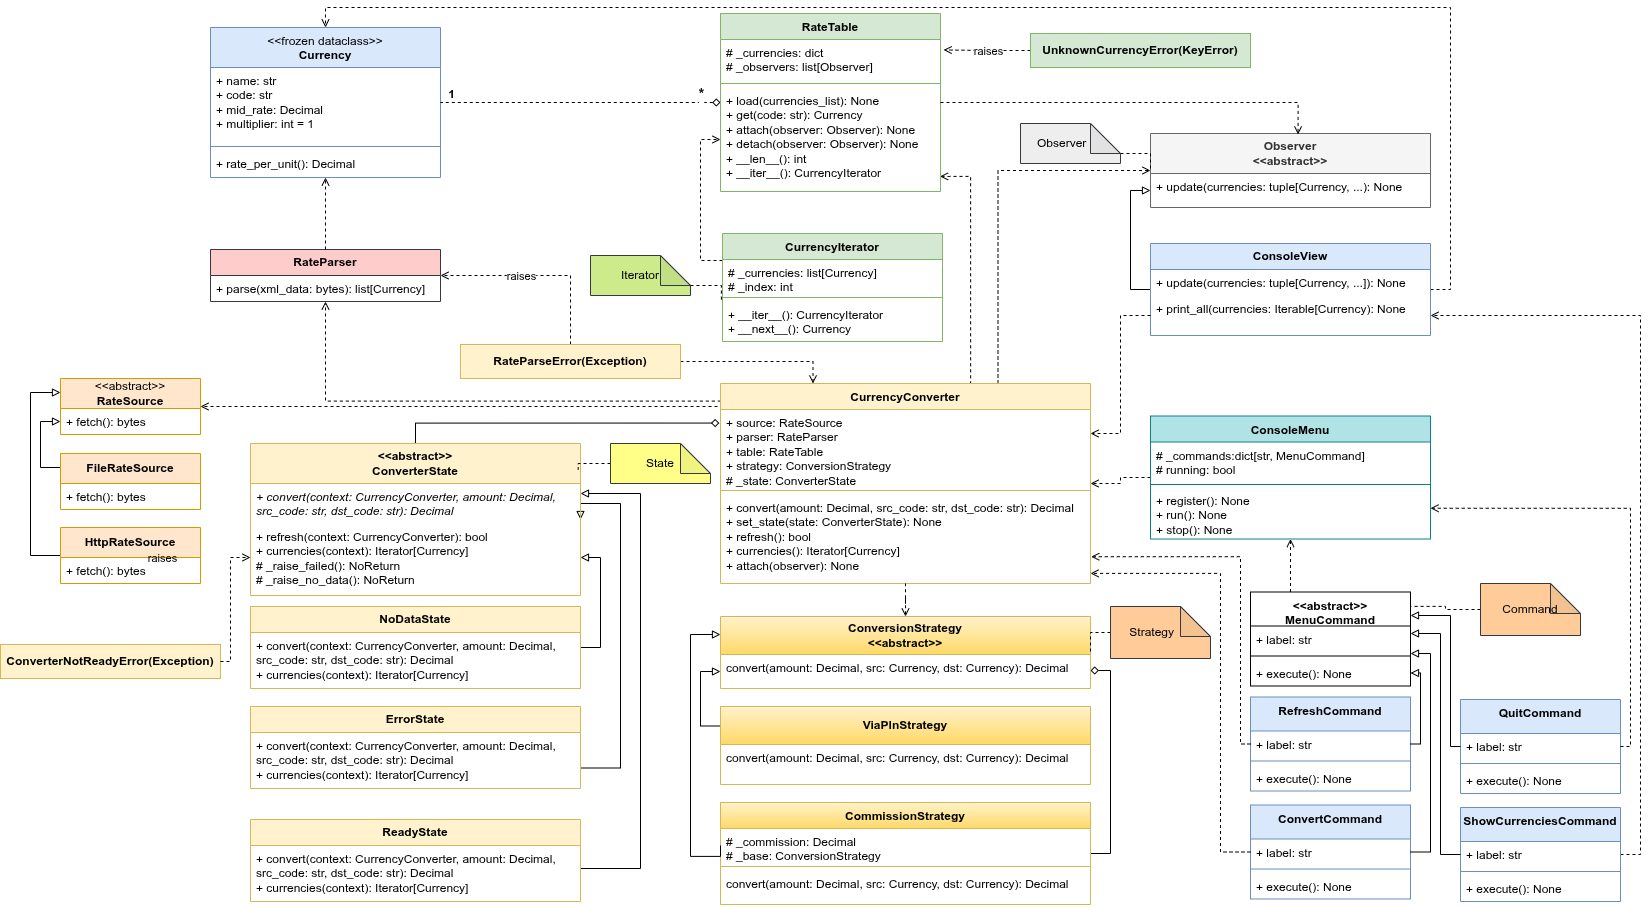
\includegraphics[width=\textwidth]{diagram.png}
    \caption{Diagram klas rozwiązania.}
    \label{fig:uml}
\end{figure}

Na diagramie wzorce zaznaczono notatkami. Warstwa interfejsu użytkownika (widok i polecenia menu) komunikuje się wyłącznie z klasą \texttt{CurrencyConverter}, która pełni rolę fasady i ukrywa przed nią tabelę kursów.

\section{Zastosowane wzorce projektowe}

\subsection{Strategia}

Wzorzec użyto w dwóch miejscach, w których istnieje kilka wymiennych sposobów wykonania tej samej czynności:
\begin{itemize}
    \item \texttt{RateSource} z implementacjami \texttt{HttpRateSource} (pobranie z internetu) i \texttt{FileRateSource} (odczyt pliku). Dzięki temu konwerter nie zależy od sposobu pozyskania danych, a testy mogą działać bez sieci,
    \item \texttt{ConversionStrategy} z implementacjami \texttt{ViaPlnStrategy} (przeliczenie przez złotego) oraz \texttt{CommissionStrategy}. Ta ostatnia przyjmuje w konstruktorze inną strategię oraz wysokość prowizji i odejmuje ją od wyniku, więc wzór przeliczania istnieje tylko w jednym miejscu.
\end{itemize}
Strategię wybiera klient z zewnątrz (w \texttt{main.py}), a konwerter korzysta wyłącznie z interfejsu.

\subsection{Stan}

Kontekstem jest \texttt{CurrencyConverter}, który deleguje metody \texttt{convert}, \texttt{currencies} i \texttt{refresh} do bieżącego obiektu stanu. Zachowanie tej samej metody zależy od fazy, w której jest konwerter:

\begin{table}[H]
    \centering
    \begin{tabular}{@{}lp{4.2cm}p{5cm}@{}}
        \toprule
        \textbf{Stan} & \textbf{convert / currencies} & \textbf{refresh} \\
        \midrule
        \texttt{NoDataState} & zgłasza \texttt{ConverterNotReadyError} (brak danych) & sukces $\rightarrow$ \texttt{ReadyState}, błąd $\rightarrow$ \texttt{ErrorState} \\
        \texttt{ReadyState} & przelicza, waliduje kwotę, zaokrągla wynik & sukces $\rightarrow$ \texttt{ReadyState}, błąd $\rightarrow$ \texttt{ErrorState} \\
        \texttt{ErrorState} & zgłasza \texttt{ConverterNotReadyError} (pobranie się nie udało) & sukces $\rightarrow$ \texttt{ReadyState}, błąd $\rightarrow$ \texttt{ErrorState} \\
        \bottomrule
    \end{tabular}
    \caption{Stany konwertera i przejścia między nimi.}
\end{table}

Bez wzorca każda metoda konwertera zawierałaby ten sam łańcuch \texttt{if/elif}, a dodanie nowego stanu wymagałoby modyfikacji klasy konwertera. Tu wystarczy dodać nową klasę stanu. Dzięki stanom użytkownik dostaje czytelny komunikat (np. ,,brak danych'') zamiast mylącego błędu nieznanej waluty przy pustej tabeli.

\subsection{Obserwator}

Podmiotem jest \texttt{RateTable}, a obserwatorem interfejs \texttt{Observer} z metodą \texttt{update}. Po każdym wywołaniu \texttt{load} tabela powiadamia wszystkich zarejestrowanych obserwatorów, przekazując im niezmienną migawkę (krotkę obiektów \texttt{Currency}). Konkretnym obserwatorem jest \texttt{ConsoleView}, który wypisuje liczbę załadowanych walut.

Tabela zna wyłącznie abstrakcyjny interfejs \texttt{Observer}, więc nie istnieje zależność cykliczna między tabelą a widokiem: widok importuje interfejs, a tabela nie importuje niczego z warstwy widoku. Dodanie drugiego obserwatora (np. rejestru historii odświeżeń) nie wymaga żadnej zmiany w \texttt{RateTable}. Rejestracja odbywa się przez metodę \texttt{attach} konwertera, który przekazuje obserwatora do tabeli.

\subsection{Iterator}

Metoda \texttt{RateTable.\_\_iter\_\_} zwraca obiekt jawnej klasy \texttt{CurrencyIterator} (z metodami \texttt{\_\_iter\_\_} i \texttt{\_\_next\_\_}), zbudowany na kopii listy walut. Wzorzec daje:
\begin{itemize}
    \item dostęp do kolejnych walut bez ujawniania, że tabela wewnętrznie jest słownikiem,
    \item osobny indeks dla każdej pętli, więc dwie pętle po tej samej tabeli nie przeszkadzają sobie,
    \item bezpieczeństwo przy ponownym wczytaniu danych w trakcie iteracji (iterator pracuje na kopii).
\end{itemize}

\subsection{Dodatkowo: Polecenie i Fasada}

Poza wymaganymi wzorcami zastosowano:
\begin{itemize}
    \item \textbf{Polecenie} w menu konsolowym: każda opcja (pokaż waluty, przelicz, odśwież, zakończ) jest osobną klasą dziedziczącą po \texttt{MenuCommand}. \texttt{ConsoleMenu} przechowuje słownik poleceń, więc nowa opcja to nowa klasa i jedna linia rejestracji, bez zmian w menu i bez łańcucha \texttt{if/elif},
    \item \textbf{Fasadę}: \texttt{CurrencyConverter} jest jedynym punktem wejścia dla interfejsu użytkownika.
\end{itemize}

\section{Zasady SOLID}

\begin{itemize}
    \item \textbf{S (Single Responsibility)}: \texttt{RateParser} tylko parsuje, \texttt{RateSource} tylko pobiera dane, strategia tylko liczy, \texttt{RateTable} tylko przechowuje i powiadamia, widok tylko wyświetla.
    \item \textbf{O (Open/Closed)}: nowe źródło danych, strategia przeliczania, stan, obserwator lub polecenie menu to nowa klasa, bez modyfikacji istniejących.
    \item \textbf{L (Liskov Substitution)}: dowolna implementacja \texttt{RateSource}, \texttt{ConversionStrategy}, \texttt{ConverterState} czy \texttt{MenuCommand} może zastąpić typ bazowy bez zmiany poprawności programu. Potwierdzają to testy z różnymi źródłami danych (plik, źródło zawodne, źródło z błędnymi danymi).
    \item \textbf{I (Interface Segregation)}: interfejsy są małe: \texttt{RateSource} i \texttt{Observer} mają po jednej metodzie, \texttt{ConversionStrategy} i \texttt{MenuCommand} po jednej metodzie roboczej. Polecenia otrzymują tylko te zależności, z których korzystają.
    \item \textbf{D (Dependency Inversion)}: \texttt{CurrencyConverter} otrzymuje źródło, parser, tabelę i strategię w konstruktorze i zależy od abstrakcji \texttt{RateSource} oraz \texttt{ConversionStrategy}. Konkretne klasy łączy dopiero \texttt{main.py}. Podobnie tabela i widok zależą od wspólnego interfejsu \texttt{Observer}, a menu od abstrakcji \texttt{MenuCommand}.
\end{itemize}

\subsection*{Ograniczenia rozwiązania}

\begin{itemize}
    \item zasada D jest spełniona częściowo: \texttt{RateParser} i \texttt{RateTable} są klasami konkretnymi, bez własnych abstrakcji,
    \item metoda \texttt{refresh} jest wspólna dla wszystkich stanów i znajduje się w klasie bazowej stanu, więc stany różnią się praktycznie metodami \texttt{convert} i \texttt{currencies},
    \item reguła zaokrąglania (dwa miejsca po przecinku) jest zapisana na stałe w \texttt{ReadyState},
    \item po nieudanym odświeżeniu konwerter przechodzi w \texttt{ErrorState}, mimo że w tabeli mogą pozostać stare kursy. Jest to świadoma decyzja: bezpieczniej zablokować przeliczanie niż liczyć na nieaktualnych danych.
\end{itemize}

\section{Obsługa błędów}

\begin{itemize}
    \item brak sieci lub pliku (\texttt{OSError}) oraz niepoprawne dane (\texttt{RateParseError}) przenoszą konwerter w \texttt{ErrorState}, a metoda \texttt{refresh} zwraca \texttt{False},
    \item parser zamienia błędy XML, brakujące pola i niepoprawne liczby na własny wyjątek \texttt{RateParseError},
    \item nieznany kod waluty zgłasza \texttt{UnknownCurrencyError},
    \item ujemna kwota zgłasza \texttt{ValueError},
    \item konwersja przed pobraniem danych lub po nieudanym pobraniu zgłasza \texttt{ConverterNotReadyError},
    \item polecenia menu przechwytują te wyjątki i wypisują czytelny komunikat, więc program nie kończy się awarią. Kwota jest wczytywana jako \texttt{Decimal}, dopuszczany jest przecinek dziesiętny, a kody walut są normalizowane do wielkich liter.
\end{itemize}

\section{Testy}

Testy jednostkowe napisano w bibliotece \texttt{pytest} i podzielono na pliki odpowiadające modułom (\texttt{test\_currency.py}, \texttt{test\_rate\_parser.py}, \texttt{test\_rate\_table.py}, \texttt{test\_conversion.py}, \texttt{test\_currency\_converter.py}, \texttt{test\_console\_view.py} i inne). Fixtury współdzielone przez kilka plików znajdują się w \texttt{conftest.py}. Testy nie korzystają z sieci: używają lokalnego pliku \texttt{sample.xml} oraz własnych źródeł testowych.

Zakres testów:
\begin{itemize}
    \item kurs jednostkowy (USD, HUF z przelicznikiem 100) i walidacja przelicznika,
    \item parser: dodanie złotego, kodowanie UTF-8 i ISO-8859-2, dane błędne (\texttt{pytest.mark.parametrize}),
    \item tabela: powiadamianie i odłączanie obserwatora, niezależność iteratorów, nieznana waluta,
    \item strategie: przeliczenia dla wielu par walut, prowizja oraz walidacja jej zakresu,
    \item konwerter: wszystkie stany i przejścia (w tym powrót z \texttt{ErrorState} dzięki źródłu zawodnemu, które za pierwszym razem zgłasza błąd), ujemna kwota, nieznana waluta, wymiana strategii,
    \item polecenia menu (z podmienionym wejściem i przechwyconym wyjściem).
\end{itemize}
Dodatkowo kod sprawdzono analizatorem typów \texttt{mypy}.

Uruchomienie testów: \texttt{pytest -v}. Uruchomienie programu: \texttt{python -m src.main}.

\section{Wnioski}

Podział na małe klasy o jednej odpowiedzialności oraz zależności skierowane ku abstrakcjom pozwoliły wymieniać źródło danych, algorytm przeliczania i interfejs użytkownika bez zmian w pozostałej części programu. Wzorzec Stan uporządkował zachowanie konwertera przy braku danych i błędach pobierania, wzorzec Obserwator rozdzielił tabelę kursów od warstwy widoku, a Iterator ukrył sposób przechowywania walut. Typ \texttt{Decimal} oraz jednokrotne zaokrąglanie na końcu obliczeń zapewniły poprawność rachunków pieniężnych. Rozwiązanie można dalej rozwijać, np. o graficzny interfejs, dodatkowe źródła danych (inne tabele NBP lub bazę danych) lub kolejnych obserwatorów.

\end{document}